\section{Сортировка массива: пузырьковая, mergesort, quicksort. Алгоритмы и оценки сложности.}


\textbf{Пузырьковая сортировка:}\\
Сложность: $O(n^2)$\\
Алгоритм: несколько раз проходимся по массиву, <<поднимая>> элемент в начало.

\textbf{Mergesort} (слияние)\\
Сложность: $T(n)=2T(\frac{n}{2})+O(n)$ или же $O(n\log n)$\\
Алгоритм: Разбиваем наш массив на 2, пока не останется по одному элементу, затем рекурсивно сравниваем каждый элемент с соседним, сортируем, объединяем.

\textbf{Quicksort}\\
Сложность в худшем случае --- $O(n^2)$, в среднем --- $O(n\log n)$\\
\textit{Алгоритм}:
\begin{enumerate}
	\item Выбрать из массива элемент, называемый опорным. Это может быть любой из элементов массива. От выбора опорного элемента не зависит корректность алгоритма, но может зависеть его эффективность.
	\item Сравнить все остальные элементы с опорным и переставить их в массиве так, чтобы разбить массив на три непрерывных отрезка, следующих друг за другом: <<элементы меньше опорного>>, <<равные>>, и <<большие>>.
	
	\item Для отрезков <<меньших>> и <<больших>> значений выполнить рекурсивно ту же последовательность операций, если длина отрезка больше единицы.
\end{enumerate}
\begin{figure}[!ht]
\centering
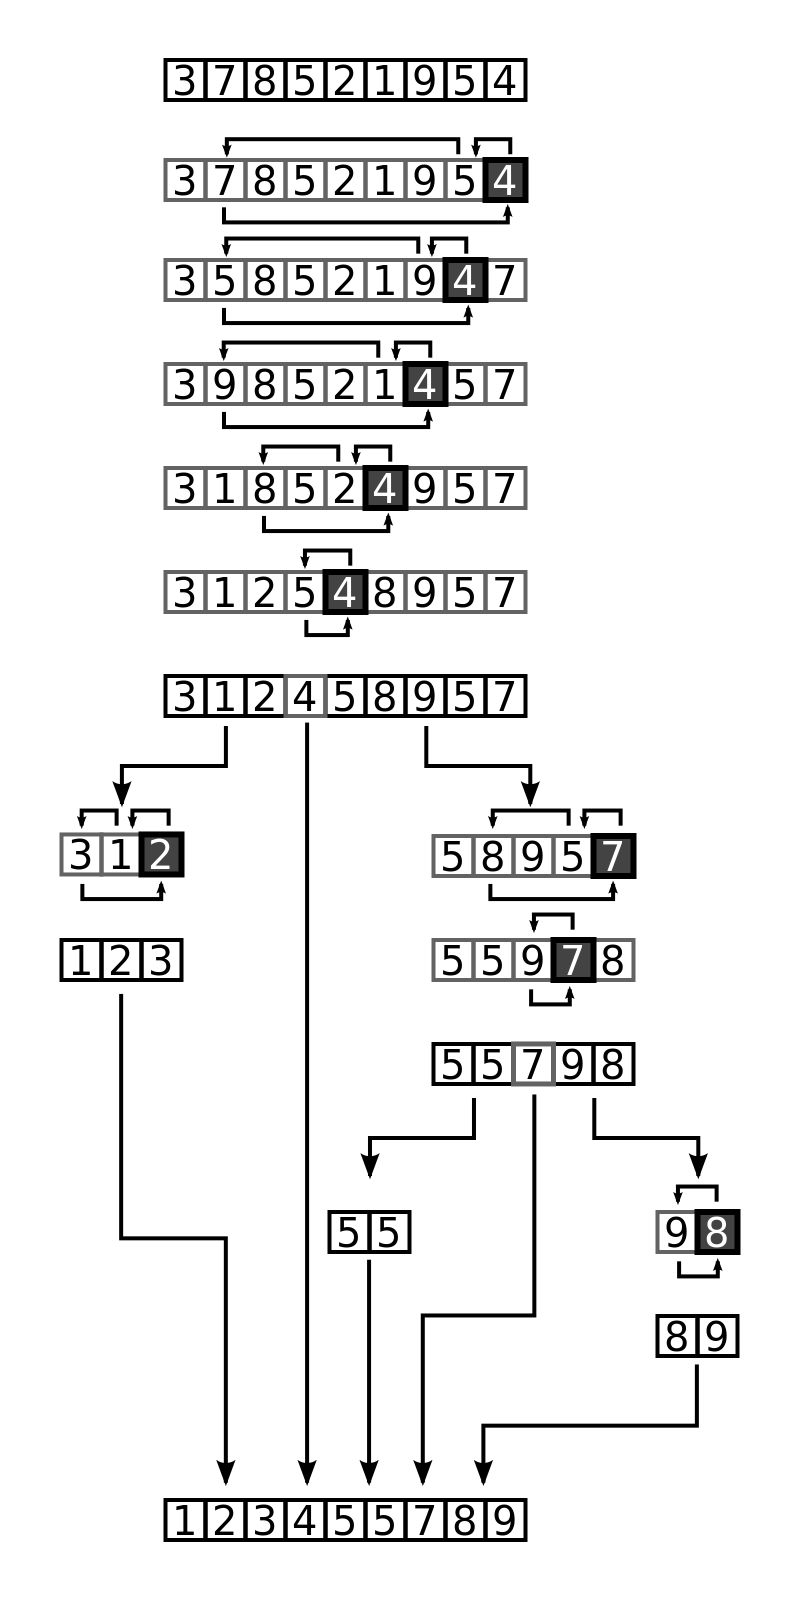
\includegraphics[width=0.2\textwidth]{img_easy/2_1.png}
\caption{\texttt{Quicksort}}
\end{figure}
